Aufbauend auf den in Kapitel \ref{kap:grundlagen} dargestellten theoretischen Grundlagen wird in diesem Kapitel die konkrete Umsetzung des LoRaWAN-basierten Tracking-Systems beschrieben. Der Schwerpunkt liegt auf der Konzeptionierung der Systemarchitektur, der Auswahl geeigneter Hardwarekomponenten sowie der Entwicklung der Software. Dabei wird insbesondere auf die Anforderungen an Modularität, Energieeffizienz und Erweiterbarkeit eingegangen. Ziel war es, ein prototypisches System zu realisieren, das als Grundlage für die spätere Analyse der Verbindungsqualität und der praktischen Einsatzmöglichkeiten dient. 
\subsection{Systemanforderungen}
Die Entwicklung des Tracking-Systems erfolgte unter der Prämisse, zunächst einen funktionsfähigen Prototypen als Proof-of-Concept zu realisieren. Dabei standen Aspekte wie Kostenoptimierung oder Robustheit im industriellen Einsatz nicht im Vordergrund. Stattdessen lag der Schwerpunkt auf Modularität und Erweiterbarkeit, um eine Plattform zu schaffen, die flexibel an unterschiedliche Szenarien angepasst werden kann. 

Als Basiskomponenten wurden eine GPS-Einheit zur Positionsbestimmung sowie eine SD-Karte zur lokalen Zwischenspeicherung vorgesehen. Externe Sensoren, beispielsweise zur Temperaturerfassung oder zur Anbindung von Sicherheitssiegeln (elektronische Plomben), sollten über modulare Schnittstellen integriert werden können. Dadurch ergibt sich eine universelle Plattform, die sich für unterschiedliche Anforderungen in der Transportlogistik anpassen lässt. 

Für die Kommunikation wurde der Einsatz von LoRaWAN spezifiziert. Aufgrund der Fokussierung auf energieeffiziente Uplink-Übertragungen ohne Bedarf an kontinuierlichen Downlinks wurde die Geräteklasse~A gewählt. Diese stellt die grundlegende und am weitesten verbreitete Gerätekategorie dar, die insbesondere für batteriebetriebene Endgeräte geeignet ist. Eine Bindung an ein spezifisches öffentliches oder privates Netzwerk wurde im Rahmen der Konzeption nicht vorgenommen, um die Flexibilität in der prototypischen Umsetzung zu wahren. 

Neben der Modularität wurde auch der Energieverbrauch als zentrale Anforderung berücksichtigt. Zwar war die Laufzeitoptimierung nicht vorrangiges Ziel der ersten Implementierung, dennoch sollte die Architektur grundsätzlich energieeffiziente Betriebsmodi unterstützen. Ergänzend dazu bietet LoRaWAN inhärente Sicherheitsmechanismen wie Ende-zu-Ende-Verschlüsselung und Schlüsselverwaltung, die für die angestrebten Einsatzszenarien als ausreichend betrachtet wurden. 

\subsection{Hardware-Design}
Für die prototypische Umsetzung des Tracking-Systems wurden zwei unterschiedliche Entwicklungsboards verwendet: das \textbf{LoRa-E5 Mini} von Seeed Studio sowie das \textbf{Heltec LoRa V2}. Beide Plattformen bieten eine gute Ausgangsbasis für eine schnelle Implementierung, unterscheiden sich jedoch in wesentlichen Aspekten, die im Rahmen der Konzeption berücksichtigt wurden.

Wie in Abbidlung \ref{fig:systemarchtektur-lora-e5-mini} zu erkennen bassiert das LoRa-E5 Mini auf einem STM32WLE5-Chip, der sowohl einen Mikrocontroller als auch ein integriertes LoRaWAN-Modul bereitstellt. Durch diese enge Integration reduziert sich die Komplexität der Schaltung, da keine externe Anbindung eines Funkmoduls erforderlich ist. Darüber hinaus verfügt das Board über einen SMA-Anschluss für externe Antennen, was die Flexibilität im Test erhöht. 

\begin{figure}[H]
\centering
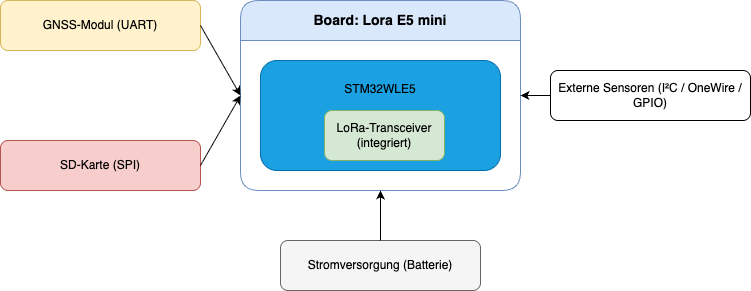
\includegraphics[scale=.5]{figures/diagrams/Architekturdiagramm_LoraE5mini.png}
\caption{Systemarchitektur Lora E5 mini}
\label{fig:systemarchtektur-lora-e5-mini}
\end{figure}

Das Heltec LoRa V2 hingegen basiert auf einem ESP32-Mikrocontroller, wie in Abbildung \ref{fig:systemarchtektur-heltec-lora-v2} zusehen, ist bei diesem Board der LoRa-Chip separat angebunden. Der ESP32 bietet zudem umfangreiche Energiesparmodi, insbesondere den Deep-Sleep-Modus, wodurch sich verschiedene Ansätze zur Laufzeitoptimierung evaluieren lassen. Zusätzlich verfügt das Board über integrierte Peripheriekomponenten wie ein OLED-Display, das für Debugging und Testzwecke nützlich war. 

\begin{figure}[H]
\centering
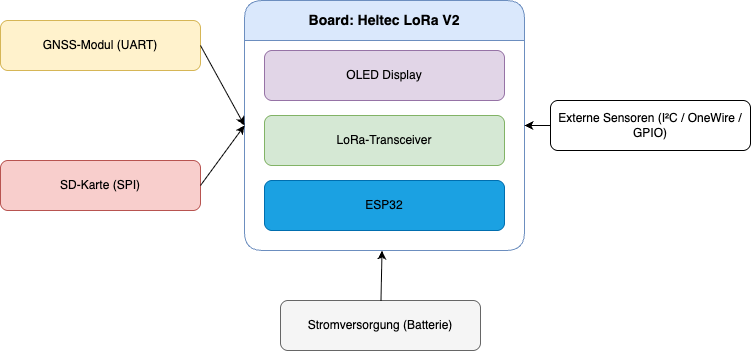
\includegraphics[scale=.5]{figures/diagrams/Architekturdiagramm_ESP32.png}
\caption{Systemarchitektur Heltec LoRa V2}
\label{fig:systemarchtektur-heltec-lora-v2}
\end{figure}

Neben den Entwicklungsboards bildeten zwei weitere Komponenten zentrale Elemente der Hardwarearchitektur:  
\begin{itemize}
    \item \textbf{GPS-Modul:} Das GNSS-Modul dient primär der Positionsbestimmung und stellt die wesentlichen Geodaten für das Tracking bereit. Darüber hinaus wird die vom Modul gelieferte Zeitinformation als Zeitbasis für das Gesamtsystem genutzt, wodurch das Gerät ohne separate Echtzeituhr über eine zuverlässige Zeitreferenz verfügt. 
    \item \textbf{SD-Karte:} Die SD-Karte wird einerseits für das lokale Logging der Messdaten eingesetzt, sodass auch bei temporären Übertragungsproblemen eine vollständige Aufzeichnung gewährleistet bleibt. Andererseits speichert sie persistente Systemparameter, wie das aktuell konfigurierte Sendeintervall sowie den LoRaWAN-Nonce-Wert, der für die sichere Teilnahme am Netzwerk erforderlich ist. Dadurch lassen sich sowohl Sicherheit als auch Reproduzierbarkeit der Übertragungen erhöhen.
\end{itemize}

Die Grundarchitektur der Prototypen sah damit eine zentrale Mikrocontroller-Einheit mit angebundener Peripherie vor. Das GPS-Modul wurde über eine UART-Schnittstelle angeschlossen, während die SD-Karte über SPI verbunden war. Weitere Sensoren, wie beispielsweise Temperatursensoren, konnten über gängige Schnittstellen wie I\textsuperscript{2}C oder OneWire ergänzt werden. 

Die Entwicklung erfolgte auf Basis von Entwicklungsboards in Verbindung mit Breadboards, wodurch eine schnelle Iteration und flexible Erweiterbarkeit möglich war. Auf die Anfertigung eigener Leiterplatten wurde im Rahmen des Proof-of-Concepts bewusst verzichtet, da der Fokus auf Funktionalität und Modularität lag und nicht auf der finalen Produktoptimierung.
\subsection{Tooling Auswahl und Software Design}
\label{sec:toolingsoftware}
Für die Entwicklung der Firmware wurde das Zephyr Real-Time Operating System (RTOS) eingesetzt. Zephyr bietet eine modulare Architektur auf Basis von Device Trees. Dies ermöglicht eine gemeinsame Codebasis für alle Microcontroler und Peripheriegeräten. Darüber hinaus stellt das Framework eine Vielzahl vorgefertigter Treiber und Bibliotheken bereit, die für die vorliegende Arbeit unmittelbar nutzbar waren. Dazu zählen unter anderem Implementierungen für LoRaWAN, UART-gebundene GPS-Module, SD-Karten mit Dateisystemunterstützung, Displays (z.\,B. OLED beim ESP32-basierten Board) sowie Schnittstellen wie OneWire und I\textsuperscript{2}C für externe Sensoren. 

Die Implementierung der Firmware erfolgte in C++, da diese Sprache im Embedded-Bereich weit verbreitet ist und ebenso einer der 3 Hauptsprache, neben C und Rust, für Zephyr RTOS ist \autocite{LanguageSupportZephyr}. Auf zusätzliche externe Libraries wurde verzichtet, da die Funktionalität durch die Zephyr-Basis bereits vollständig abgedeckt war. \\

Das Software-Design folgt einem modularen Ansatz: Für jede Komponente existiert ein eigenständiges Modul, das während des Systemstarts initialisiert wird. Hierzu gehören insbesondere die SD-Karte, das GPS-Modul sowie beliebige Sensorschnittstellen. Alle implementierten externen Sensoren besitzen eine einheitliche \texttt{read()}-Methode, über die Messwerte ausgelesen werden können. Die Auswahl und Aktivierung einzelner Module erfolgt über die Projektkonfiguration in der Datei \texttt{prj.conf}. Auf diese Weise kann beispielsweise über den Eintrag:
\begin{verbatim}
lora_wan_tracker_temp_sensor=y
\end{verbatim}
die Einbindung eines Temperatursensors aktiviert werden. Dieser Ansatz ermöglicht eine flexible Anpassung der Firmware an unterschiedliche Anwendungsfälle, ohne tiefgreifende Änderungen am Quellcode vorzunehmen.

Ein Bestandteil des Software-Designs ist die Datenpaketstruktur, mit der die gesammelten Messwerte über LoRaWAN übertragen werden. Jedes Paket enthält zunächst die GPS-Daten und den Zeitstempel des Geräts in komprimierter Form. Hierzu werden Breiten- und Längengrad, Höhe, Genauigkeit sowie die Anzahl empfangener Satelliten als Big-Endian-Werte in ein Byte-Array codiert.

Im Anschluss an die GPS-Daten und Zeitdaten wird ein 4-Bit-Feld angefügt, das als Bitmap fungiert. Jedes Bit steht für einen spezifischen Sensor und zeigt an, ob für diesen Sensor Messwerte im aktuellen Paket enthalten sind. Die eigentlichen Sensordaten folgen in einer festgelegten Reihenfolge. Diese Struktur erlaubt eine flexible Erweiterung, da neue Sensortypen durch die Definition zusätzlicher Bits in der Bitmap ergänzt werden können, ohne die bestehende Protokollstruktur zu verändern. Eine Vollständige ansicht des Paketes kann Abbildung \ref{fig:lorawanPacket} entnommen werden.

\begin{figure}[H]
\centering
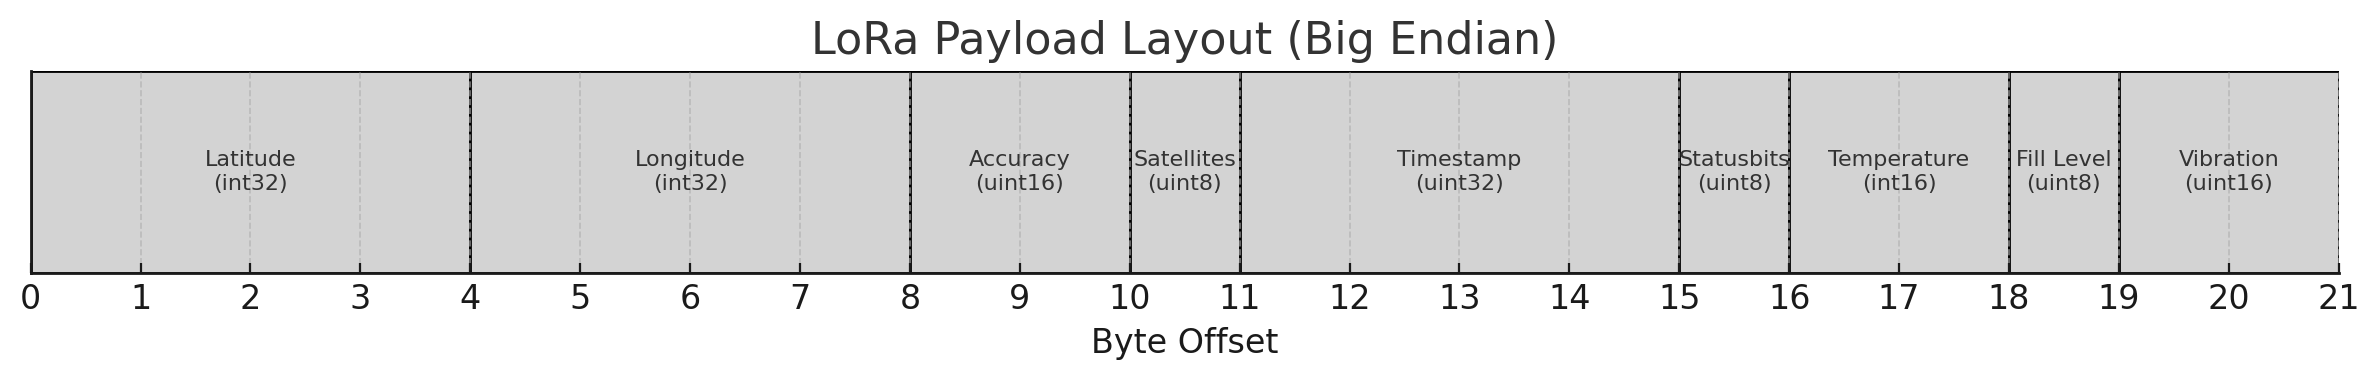
\includegraphics[scale=.5]{figures/asstes/lorawan-packet-layout.png}
\caption{Datensegment des LoraWAN Pakets}
\label{fig:lorawanPacket}
\end{figure}

Auf der Seite des LoRaWAN Network Servers (LNS) wird das Datenpaket mittels JavaScript entschlüsselt. Die dort implementierte Routine interpretiert die Bitfolge und überführt die enthaltenen Werte in ein JSON-Format, welches dann für nachgelagerte Anwendungen, wie Visualisierung oder Analyse, weiterverarbeitet werden kann. 

Die gewählte Architektur vereint damit eine modulare Firmwarestruktur, die sich flexibel anpassen lässt, mit einer kompakten und erweiterbaren Datenrepräsentation, die für den Einsatz in ressourcenbeschränkten IoT-Geräten optimiert ist.
\subsection{Implementierung}
Im nachfolgenden soll die Implementierung des LoraWAN-Trackers beschrieben werden. Dabei wird der Systemstart und die Initialisierung der einzelnen Komponennten sowie der Datenpfad und das Paketfromat beschreiben. Des weiteren wird der Netzbeitritt so wie das Senden der Pakete erklärt. Auch wird beschreiben wie das Gerät Konfiguriert werden kann sowie die Interaktion mit der Shell bschrieben. Zuletzt soll noch drauf eingegangen werden wie die Fehlerbehandlung sowie das Logging funktioniert.

\paragraph*{Systemstart und Initialisierung}
Beim Start initialisiert die Firmware die Subsysteme in fester Reihenfolge: Shell, LED/GPIO, SD-Karte (FATFS, Mount-Punkt \texttt{/SD:}), GNSS-UART, LoRaWAN-Stack. Das LoRaWAN-Subsystem wird über die Zephyr-API gestartet und anschließend für EU868 konfiguriert. Ebenso wird ADR ist aktiviert. Die SD-Karte wird über das Disk-Access-API angebunden und als FATFS eingehängt. GNSS läuft als NMEA-Quelle am konfigurierten UART mit Callback-Registrierung.

\paragraph*{Datenpfad und Paketformat}
GNSS-Daten werden über einen Callback gelesen, aufbereitet und in eine kompakte Payload kodiert der genaue Aufbau des einzelnen Pakets wurde in Abschnitt \ref{sec:toolingsoftware} erklärt. Breite und Länge als \texttt{int64} big-endian, Höhe \texttt{int32}, Genauigkeit \texttt{uint16}, Satelliten \texttt{uint8}. Die Kodierung erfolgt in ein Byte-Array fester Länge. Die Position wird nur bei gültigem Fix versendet.

\paragraph*{Netzbeitritt und Senden}
Der Netzbeitritt nutzt OTAA (wie in Abschnitt \ref{sec:joinmechanissmus_otaa} Join-Mechanismus (OTAA)  erklärt). Die Join-Parameter (\texttt{dev\_eui}, \texttt{join\_eui}, \texttt{app\_key}) werden je nach Zielnetz, TTN oder Helium, gesetzt. Der \texttt{dev\_nonce} wird persistent verwaltet und vor jedem Join erhöht. Nach erfolgreichem Join sendet das Gerät bestätigte Uplinks (\texttt{CONFIRMED}) auf Port~2.

\paragraph*{Persistenz und Konfiguration}
Sendeintervall (\texttt{/SD:/int.txt}) und LoRaWAN-Nonce (\texttt{/SD:/nonce.txt}) sind persistent gespeichert. Beide werden beim Start gelesen. Das Intervall kann zur Laufzeit über die Shell gesetzt werden und wird sofort wirksam. Dateioperationen nutzen Zephyrs VFS und FATFS-Implementierung.

\paragraph*{Shell-Befehle}
Die Shell implementiert Befehle zum Setzen des Sendeintervalls sowie zum Abfragen von Positiondaten über das GPS modul. Ebenso kann ein Zähler der erfolgreicher Übertragungen ausgelesen werden. Die Implementierung verwendet das Zephyr-Shell-Subsystem mit statischen Kommandoregistrierungen.

\paragraph*{Fehlerbehandlung und Logging}
Wenn der Tracker in einen Fehlerzustand läuft wird das durch eine blinkende LED-Schleife auf dem jeweiligen Dev-Board signalisiert. Jede Sendeoperation wird mit Positionsdaten, RSSI/SNR (falls vorhanden) und Erfolgsflag in \texttt{/SD:/log.txt} protokolliert, um spätere Auswertungen zu ermöglichen. Downlink-Metadaten werden über einen registrierten Downlink-Callback erfasst.
\subsection{Anwendungslogik}
Das Tracking Gerät hat zwei grundlegende Betriebsmodi die im Nachfolgenden kurz erläuchtert werden sollen:

\begin{itemize}
    \item \textbf{Periodisches Senden:} 
    Daten werden in festen Zeit Intervallen übermittelt (z.\,B. alle 5, 15 oder 60 Minuten). 
    Dieser Ansatz ist einfach und sorgt für eine kontinuierliche Nachverfolgbarkeit über die Transportstrecke. 
    Allerdings steigt der Energieverbrauch deutlich mit kürzer werdenden Intervallen \cite{lansitec2024lorawan,cloudstudio2023lorawan}.
    
    \item \textbf{Ereignisgesteuertes Senden:} 
    Eine Übertragung erfolgt nur bei bestimmten Ereignissen, etwa beim Öffnen einer Plombe, Überschreiten eines Temperaturgrenzwertes 
    oder bei Erschütterung des Transportguts. 
    Dadurch lässt sich die Batterielaufzeit zwar signifikant verlängern, jedoch sind die Positionsdaten zwischen den Ereignissen lückenhaft 
    \cite{tektelic2023assettracking,zhang2022lorawanmac}.
\end{itemize}

Am besten geeignet ist desswegen ein Hybrieder Ansatzt. Dabei sollen regelmäßige Intervall-Updates mit großen Intervallen mit zusätzlichen Ereignisübertragungen kombiniert werden. 
Dadurch kann eine Balance zwischen Energieeffizienz und Transparenz der Transportüberwachung erreicht werden.
\subsection{Energiemanagement und Batterielaufzeit}
Die Herstellerangaben der wesentlichen Komponenten sind in Tabelle \ref{tab:stromverbrauch} zusammengefasst. 
Für jede Betriebsart sind typische Ströme aufgeführt. Ebenso wurden eigene Messungen angestellt um die bestehenden Werte zu validieren.

\begin{table}[H]
\centering
\scriptsize
\begin{tabular}{|l|l|c|c|}
\hline
\textbf{Komponente} & \textbf{Modus} & \textbf{Strom Datenblatt} & \textbf{Messung} \\ \hline
LoRa-E5 Mini & DS & 2,1 $\mu$A \cite{stm32wl} & ... \\ \hline
 & TX 22 dBm & 122 mA \cite{seeed_lorae5} & ... \\ \hline
 & RX & 5,5 mA \cite{seeed_lorae5} & ... \\ \hline
Heltec ESP32 V2 & DS & 10 $\mu$A \cite{esp32_datasheet} & ... \\ \hline
 & MCU aktiv & 20--80 mA \cite{esp32_datasheet} & ... \\ \hline
 & LoRa TX 20 dBm & 120 mA \cite{sx1276_datasheet} & ... \\ \hline
GPS (NEO-6M/ATGM336H) & Acquisition & 45 mA \cite{ublox_neo6m} & ... \\ \hline
 & Tracking & 25 mA \cite{ublox_neo6m} & ... \\ \hline
SD-Karte & Idle & 0,2--0,4 mA \cite{sandisk_sd} & ... \\ \hline
 & Write & 30--100 mA \cite{sandisk_sd} & ... \\ \hline
DS18B20 & Conversion & 1,5 mA \cite{ds18b20} & ... \\ \hline
 & Standby & $<$1 $\mu$A \cite{ds18b20} & ... \\ \hline
MPU-6050 & Aktiv & 3,9 mA \cite{mpu6050} & ... \\ \hline
 & Sleep & 8 $\mu$A \cite{mpu6050} & ... \\ \hline
OLED (Heltec) & On & 20--30 mA \cite{heltec_doc} & ... \\ \hline
Plombe (GPIO) & Idle & $<$1 $\mu$A & ... \\ \hline
\end{tabular}
\caption{Stromaufnahme der Komponenten.}
\label{tab:stromverbrauch}
\end{table}